\documentclass[12pt,a4paper,twoside]{article}
\usepackage[utf8]{inputenc}
\usepackage{setspace}
\usepackage{hyperref}
\usepackage[english]{babel}
\usepackage[nobiblatex]{xurl}
\usepackage{url}
\usepackage{graphicx}
\usepackage[left=3.5cm,right=2.5cm,top=2.5cm,bottom=2.5cm]{geometry}
\usepackage{fancyhdr}
\usepackage{float}

% Header and Footer
\pagestyle{fancy}
\fancyhead{} % clear header
\fancyfoot{}  % clear footer
\fancyfoot[LE,RO]{\thepage}
\renewcommand{\headrulewidth}{0pt}
\renewcommand{\footrulewidth}{0pt}

\renewcommand{\baselinestretch}{1.5} 

\begin{document}

\fontsize{14pt}{14pt}\selectfont
\begin{titlepage}
 \begin{center}
       Computer Science\\
       Akademia WSB\\
       Poland\\

      \vspace*{2cm}

      
\includegraphics[width=0.4\textwidth]{images-aws/university}

       \vspace*{3cm}
      
       \textbf{Subject: Corporate IT Infrastructure Project}
 
       \begin{center}
	\Large\textbf{Implementation of Github and Jenkins \\ as CI / CD}\\
       \end{center}

       \vspace{0.5cm}
        
            
       \vspace{1.5cm}


       \mbox{}\hfill \textbf{Lecture:}  dr inż. Paweł Świtała

       {\raggedleft \textbf{Students:} Roman Tymochko, \par}
       {\raggedleft Dmitri Cerevatov,       \par}
       {\raggedleft Ioan Zîcu                    \par}


       \vfill
            

       \vspace{2cm}
     
       2020
            
   \end{center}
\end{titlepage}

\newpage

\fontsize{12pt}{12pt}\selectfont


\section{Setup AWS EC2 Instance}

\subsection{Create a Security Group for Amazon EC2 Instance}

We will create a security group and add the following rules:
\begin{itemize}
	\item Allow inbound HTTP access from anywhere
	\item Allow inbound SSH traffic from a specific computer's public IP address in order to connect to the instance
\end{itemize}


1. First of all we open the Amazon EC2 console \url{ https://console.aws.amazon.com/ec2/} 


2. In the navigation bar, we select \textbf{US West (Oregon)} region. This region use the Amazon EC2 console that is the newest version. If we select regions from Europe, then it will be available just Amazon VPC console, the older version.


\begin{figure}[H]
    \centering
        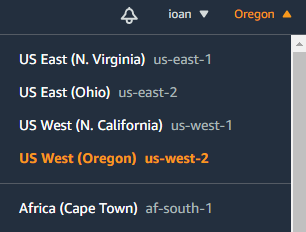
\includegraphics[width=7cm]{images-aws/1-aws-zone.png}
        \caption{AWS - select US West Zone}
\end{figure}


3. In the left-hand navigation bar, we choose the \textbf{Security Groups}, and then click on \textbf{Create Security Group}.


4. We name our Security Group \textbf{WebServerSecurityGroup} and select the VPC from the list.


5. In the \textbf{Inbound} tab, we add the following rules:
\begin{itemize}
	\item \textbf{HTTP} with source address 0.0.0.0/0 (basically open to any) and 46.187.163.63/32 (public IP address of the administrator)
	\item Open \textbf{port 8080} with source address 0.0.0.0/0 (basically open to any) and 46.187.163.63/32 (public IP address of the administrator)
	\item \textbf{SSH}   source address 46.187.163.63/32 - just administrator to be able to access the instance via SSH.
	\item \textbf{HTTPS} with source address 0.0.0.0/0 (basically open to any) and 46.187.163.63/32 (public IP address of the administrator)
\end{itemize}


\begin{figure}[H]
    \centering
        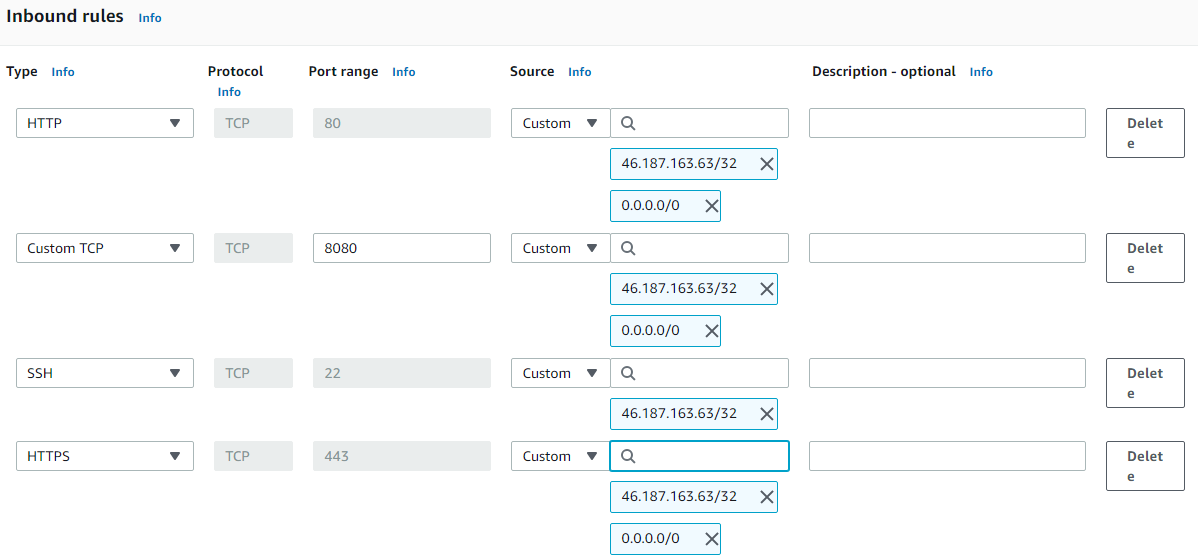
\includegraphics[width=15cm]{images-aws/3-inbound-rules.png}
        \caption{Setup rules for the inbound traffic}
\end{figure}


6. Then we click \textbf{Create}.


\begin{figure}[H]
    \centering
        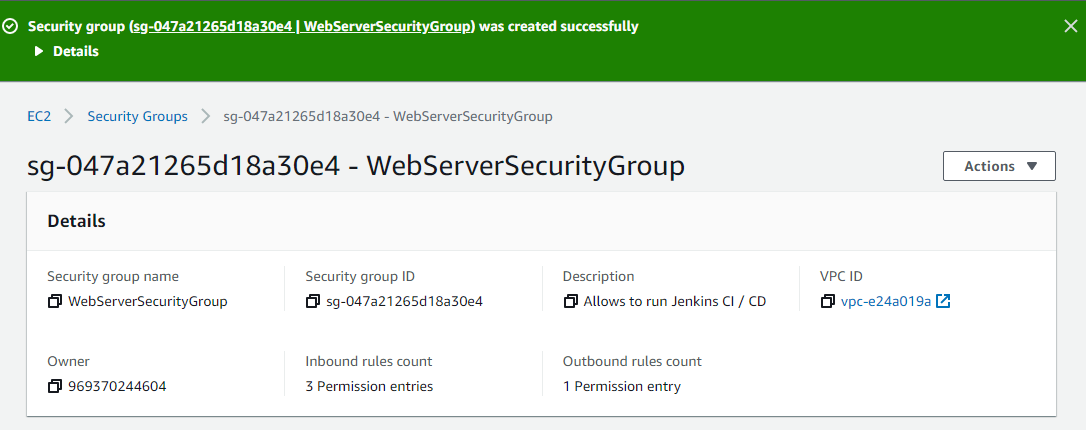
\includegraphics[width=15cm]{images-aws/12-create-sg-created.png}
        \caption{Security Group was successfully created}
\end{figure}


~\newpage

\subsection{Launch the Amazon EC2 Instance}


1. In the left-hand navigation bar of the Amazon EC2 console, we select \textbf{Instances}, and click \textbf{Launch Instance}.


\begin{figure}[H]
    \centering
        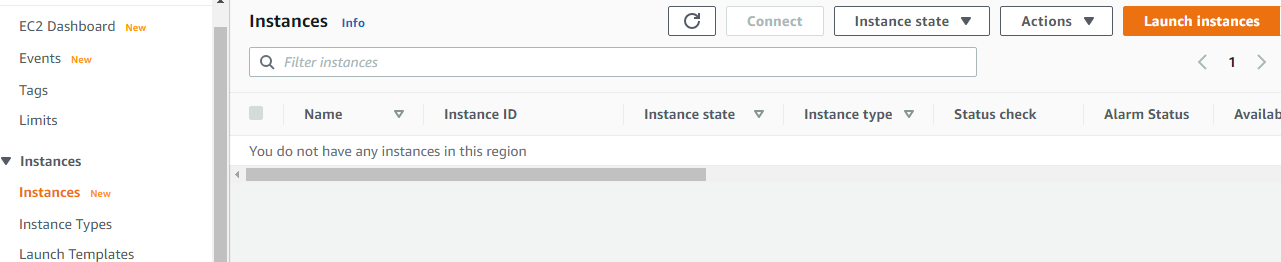
\includegraphics[width=15cm]{images-aws/4-instances.png}
        \caption{Navigate to the Instances Menu}
\end{figure}


2. On the \textbf{Choose an Amazon Machine Image page}, we select an Amazon Linux AMI with the HVM virtualization type.


\begin{figure}[H]
    \centering
        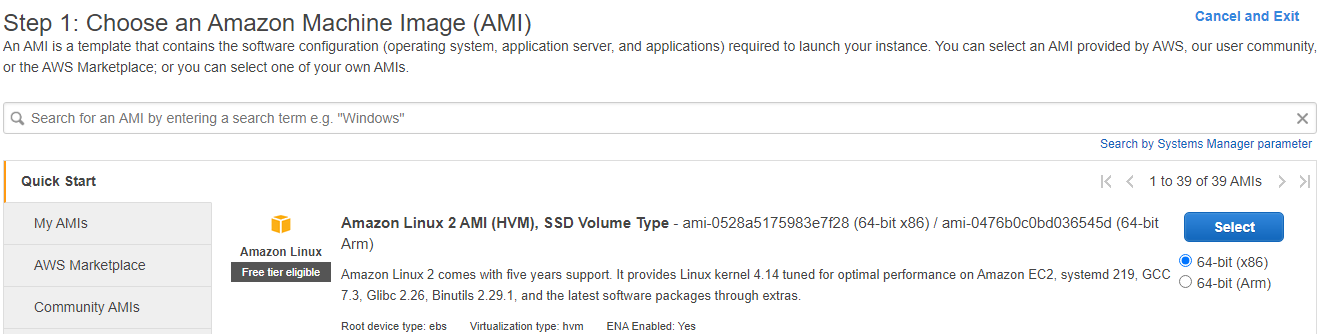
\includegraphics[width=15cm]{images-aws/5-amazon-linux.png}
        \caption{Choose Amazon Linux 2 AMI Virtual Machine}
\end{figure}


3. On the \textbf{Choose an Instance Type} page, the \textbf{t2.micro} instance is selected by default. We keep this instance type to stay within the free tier.


4. Then we click \textbf{Next: Configure Instance Details}


\begin{figure}[H]
    \centering
        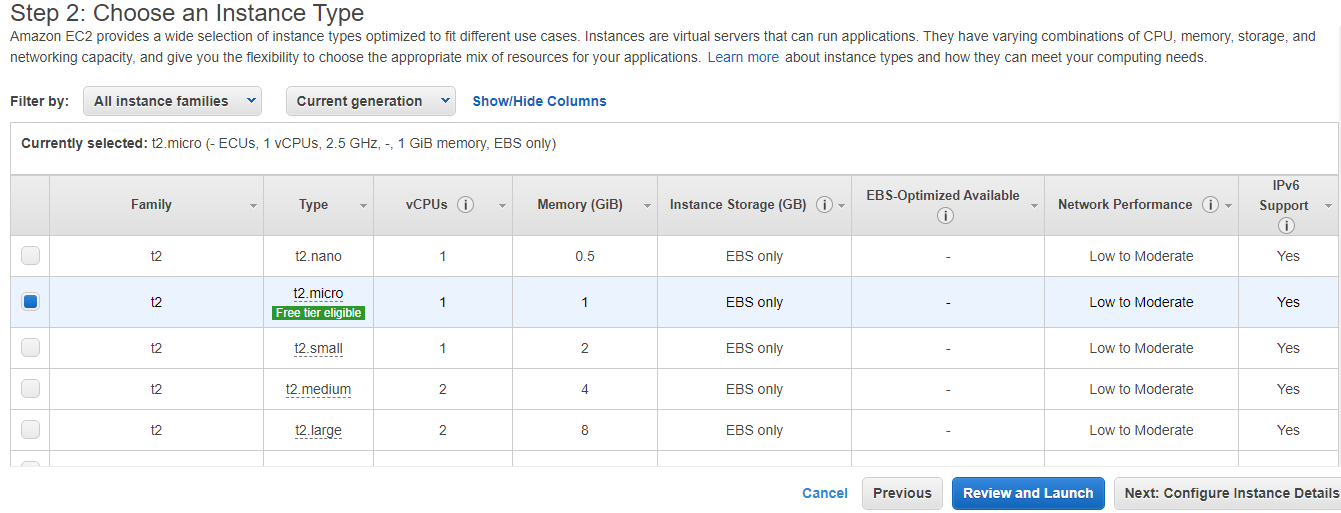
\includegraphics[width=15cm]{images-aws/6-instance-type.png}
        \caption{Choose t2.micro Instance, Free Tier}
\end{figure}


5. On the \textbf{Configure Instance Details} page we do the following:


\begin{itemize}
	\item From the \textbf{Network} we choose the VPC, and from \textbf{Subnet} we choose the \textbf{public} subnet.
	\item We ensure that in the \textbf{Auto-assign Public IP} the option \textbf{Enable} is selected. Otherwise the instance will not
get a public IP address or a public DNS name.
	\item Click \textbf{Review and Launch}.
\end{itemize}


\begin{figure}[H]
    \centering
        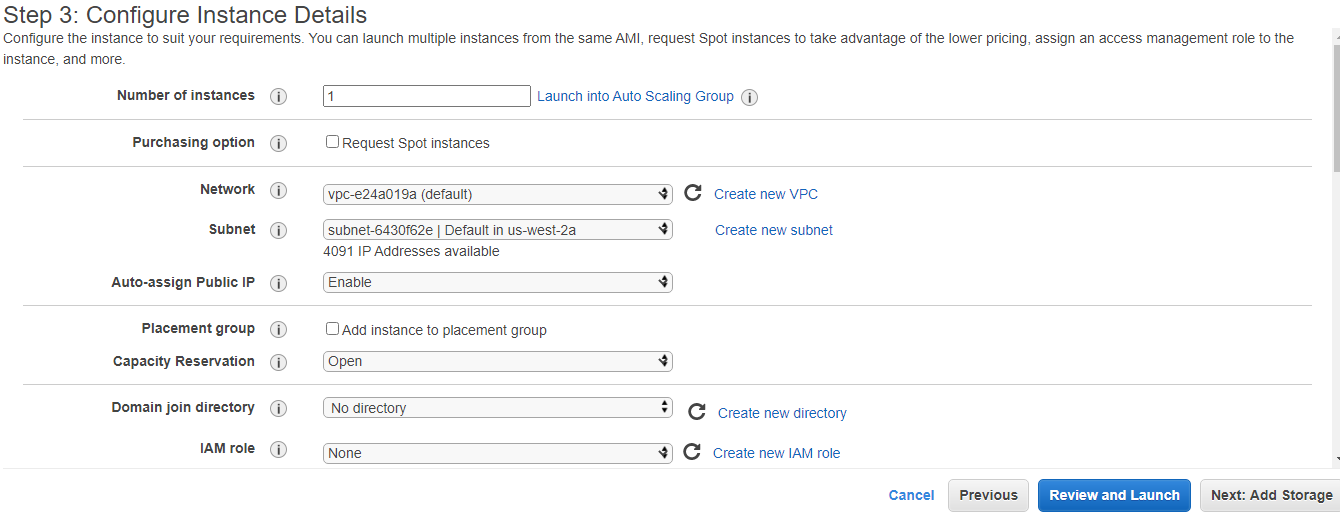
\includegraphics[width=15cm]{images-aws/7-config-instance-details.png}
        \caption{Configure Instance Details}
\end{figure}


6. On the \textbf{Review and Launch} page we click \textbf{Edit security groups}.


7. On the \textbf{Configure Security Group} page we select the \textbf{WebServerSecurity Group} that we created and then click \textbf{Review and Launch}.


\begin{figure}[H]
    \centering
        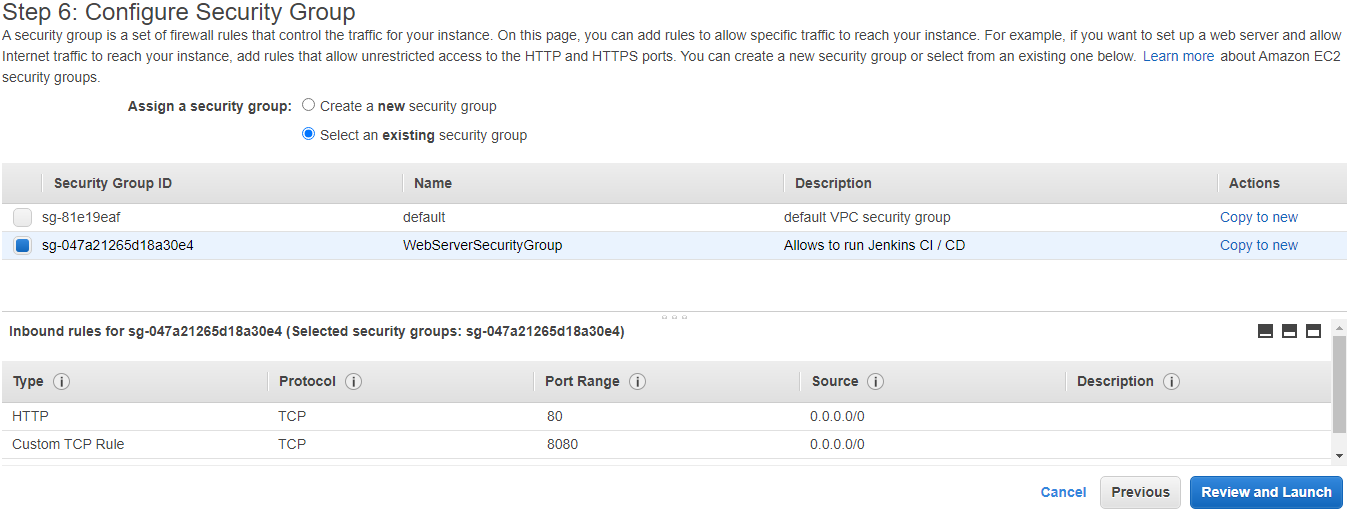
\includegraphics[width=15cm]{images-aws/8-config-sec-group.png}
        \caption{Configure Security Group}
\end{figure}


8. On the \textbf{Review Instance Launch} page, we click \textbf{Launch}.


\begin{figure}[H]
    \centering
        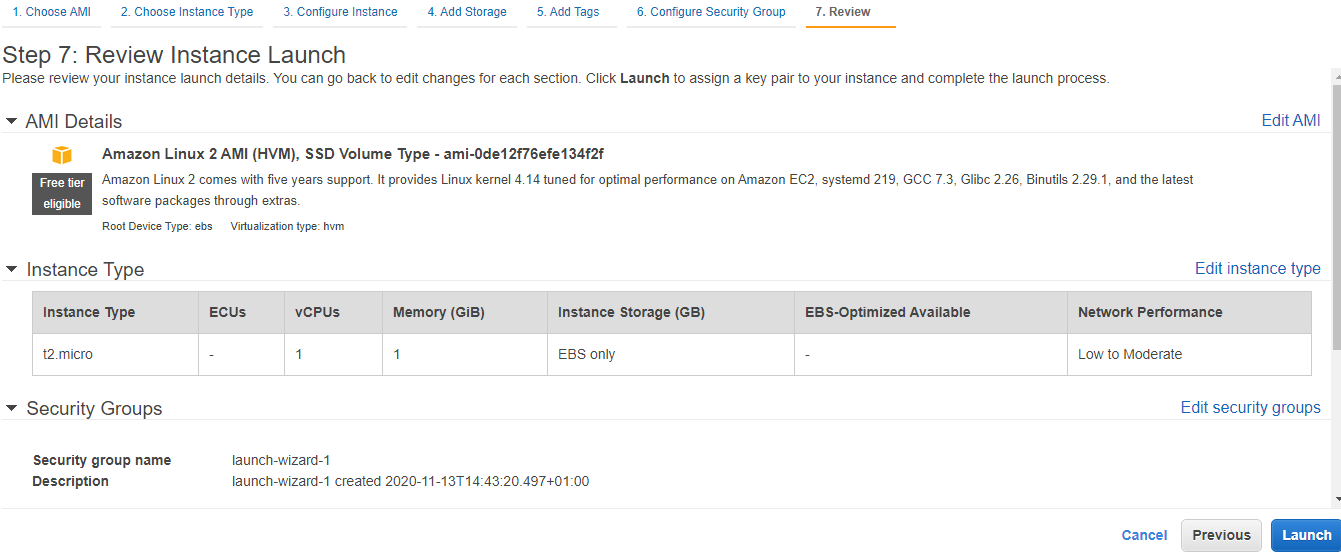
\includegraphics[width=15cm]{images-aws/9-review-instance-launch.png}
        \caption{Review Instance Launch}
\end{figure}


9. Next, in the \textbf{Select an existing key pair or create a new key pair} dialog box, we select \textbf{Create a new key pair} and enter the name. After creating the key in .pem format we will be able to access the instance via SSH.


\begin{figure}[H]
    \centering
        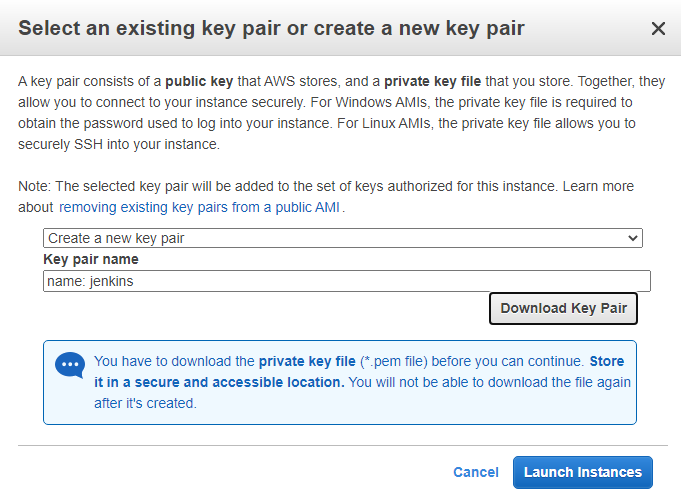
\includegraphics[width=8cm]{images-aws/10-key-pair.png}
        \caption{Create a new key pair}
\end{figure}


10. Click on the \textbf{Launch Instances} button.


\begin{figure}[H]
    \centering
        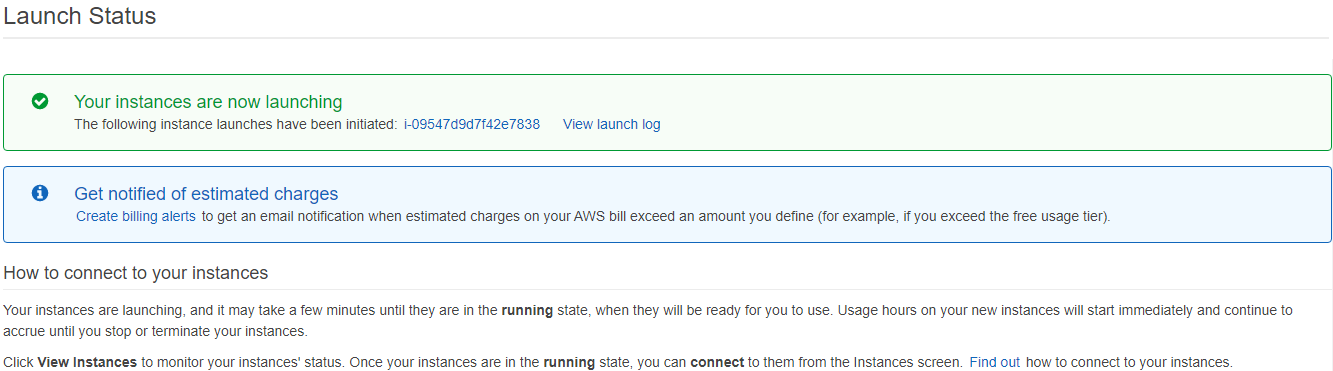
\includegraphics[width=15cm]{images-aws/11-launch-status.png}
        \caption{Launch Status}
\end{figure}


We make sure that the instance is up and running.


\begin{figure}[H]
    \centering
        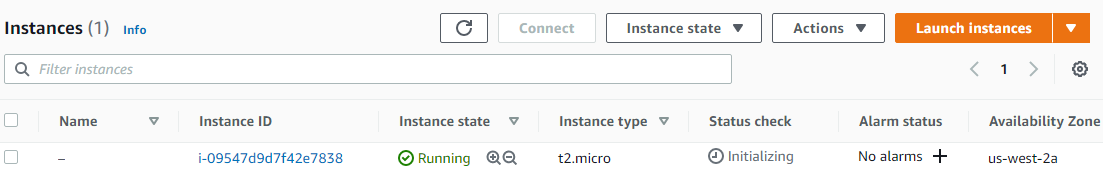
\includegraphics[width=15cm]{images-aws/13-running-instance.png}
        \caption{Verify Running Instance}
\end{figure}



~\newpage


\section{Install and Configure Jenkins}


\subsection{Connect to the EC2 Instance using SSH}


After the instance was launched, we can connect to it and use it via SSH bash shell. For this purpose we will use the \textbf{Git Bash} tool.


1. From \textbf{Git Bash} we use the \textbf{ssh} command to connect to the instance. We specify the private key (.pem) file and the ec2-user@public\_dns\_name.

\begin{verbatim}
ssh -i namejenkins.pem 
ec2-user@ec2-52-12-213-243.us-west-2.compute.amazonaws.com
\end{verbatim}

\begin{figure}[h!]
    \centering
        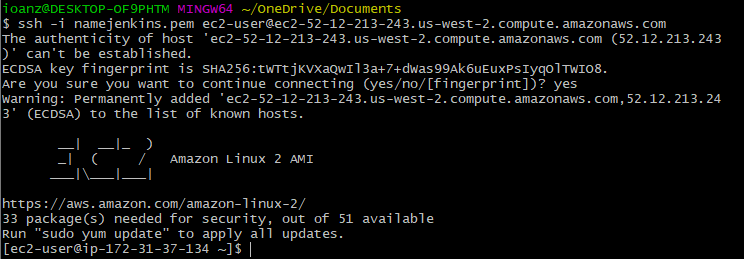
\includegraphics[width=15cm]{images-aws/14-ssh-connect.png}
        \caption{SSH into Amazon Linux 2 AMI}
\end{figure}


\subsection{Download and Install Jenkins}


1. We first ensure that the software packages are up to date.


\begin{verbatim}
sudo yum update -y
\end{verbatim}

\begin{figure}[h!]
    \centering
        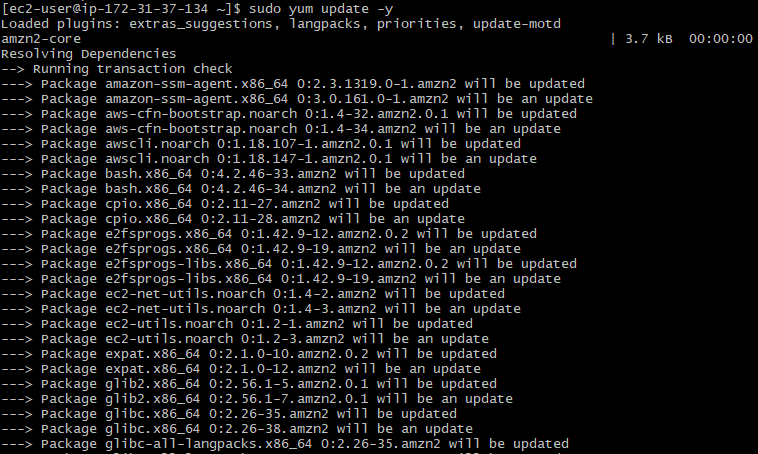
\includegraphics[width=15cm]{images-aws/15-yum-update.png}
        \caption{Update packages}
\end{figure}


2. The Jenkins will require Java JDK, so we install it on the EC2 instance.

\begin{verbatim}
sudo yum install java-1.8.0-openjdk
\end{verbatim}

\begin{figure}[h!]
    \centering
        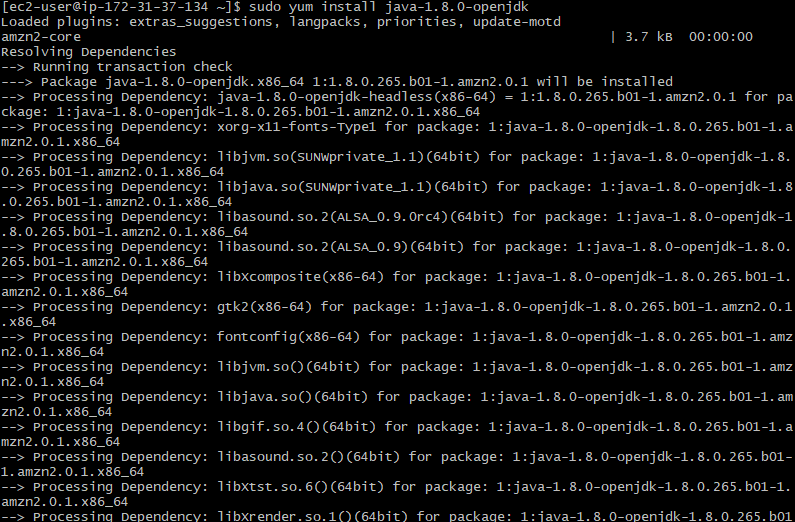
\includegraphics[width=15cm]{images-aws/20-install-java.png}
        \caption{Install Java Open JKD}
\end{figure}

3. We add the Jenkins repository using the following command:

\begin{verbatim}
sudo wget -O
/etc/yum.repos.d/jenkins.repo http://pkg.jenkins-
ci.org/redhat/jenkins.repo
\end{verbatim}

\begin{figure}[h!]
    \centering
        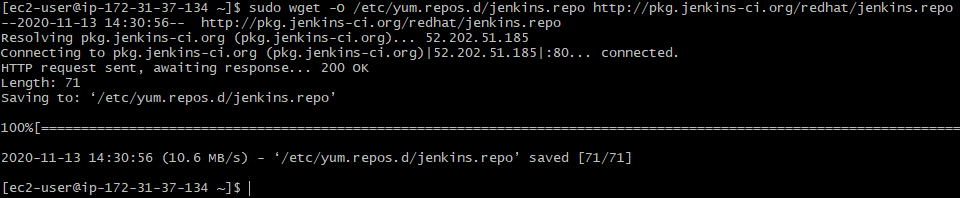
\includegraphics[width=15cm]{images-aws/16-download-jenkins.png}
        \caption{Add the Jenkins repository}
\end{figure}

4. Import a key file from Jenkins-CI to enable installation from the package:

\begin{verbatim}
sudo rpm --import
https://pkg.jenkins.io/redhat/jenkins.io.key
\end{verbatim}

\begin{figure}[h!]
    \centering
        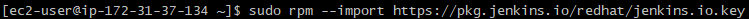
\includegraphics[width=15cm]{images-aws/17-import-jenkins-keys.png}
        \caption{Import Jenkins official keys to enable installation from the package}
\end{figure}

5. Install Jenkins:

\begin{verbatim}
sudo yum install jenkins -y
\end{verbatim}

\begin{figure}[h!]
    \centering
        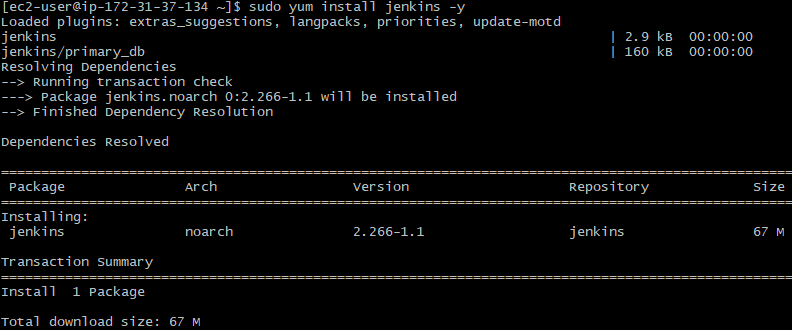
\includegraphics[width=15cm]{images-aws/18-install-jenkins.png}
        \caption{Install Jenkins}
\end{figure}

6. Start Jenkins as a service:

\begin{verbatim}
sudo service jenkins start
\end{verbatim}

\begin{figure}[h!]
    \centering
        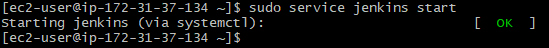
\includegraphics[width=11cm]{images-aws/21-start-jenkins.png}
        \caption{Start the Jenkins Service}
\end{figure}



\newpage

\subsection{Configure Jenkins}

Jenkins is now available and running on the EC2 instance. To configure Jenkins we:


1. Connect to the \url{http://ec2-52-12-213-243.us-west-2.compute.amazonaws.com:8080/} using Chrome browser.
Then we will be able to access the Jenkins management interface.


\begin{figure}[h!]
    \centering
        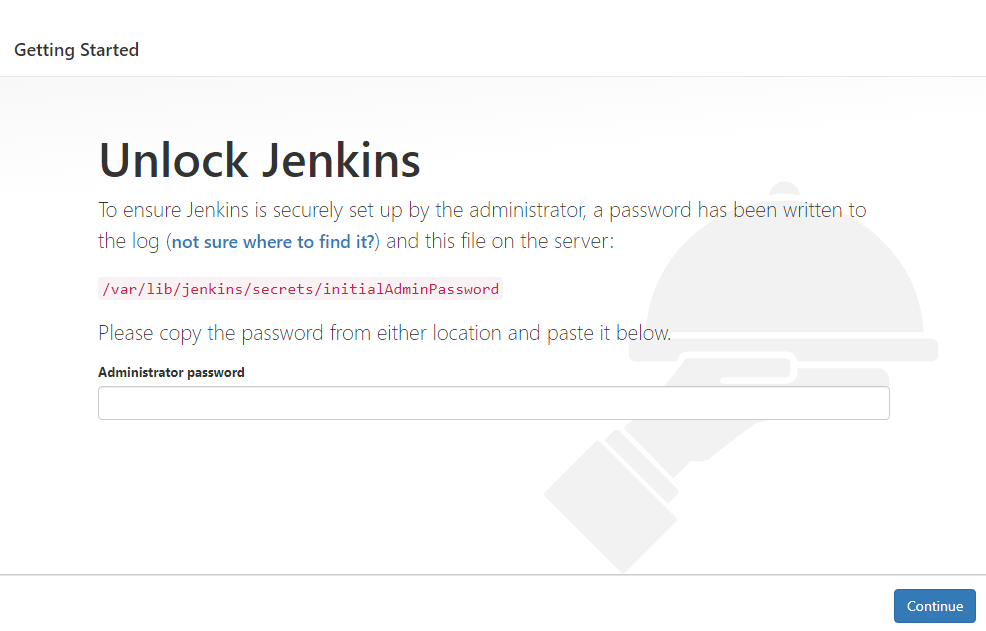
\includegraphics[width=15cm]{images-aws/22-unlock-jenkins.png}
        \caption{Unlock Jenkins}
\end{figure}


2. We print on the console the initial admin password found in \textbf{/var/lib/jenkins/secrets/initialAdminPassword}, using the following command:


\begin{verbatim}
sudo cat
/var/lib/jenkins/secrets/initialAdminPassword
\end{verbatim}


\begin{figure}[h!]
    \centering
        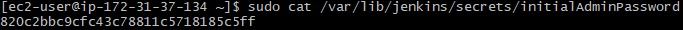
\includegraphics[width=13cm]{images-aws/23-get-jenkins-admin-pass.png}
        \caption{Get initial Admin Password}
\end{figure}


3. The Jenkins installation script directs to the \textbf{Customize Jenkins} pages. We click on the  \textbf{Install suggested plugins}.

\begin{figure}[h!]
    \centering
        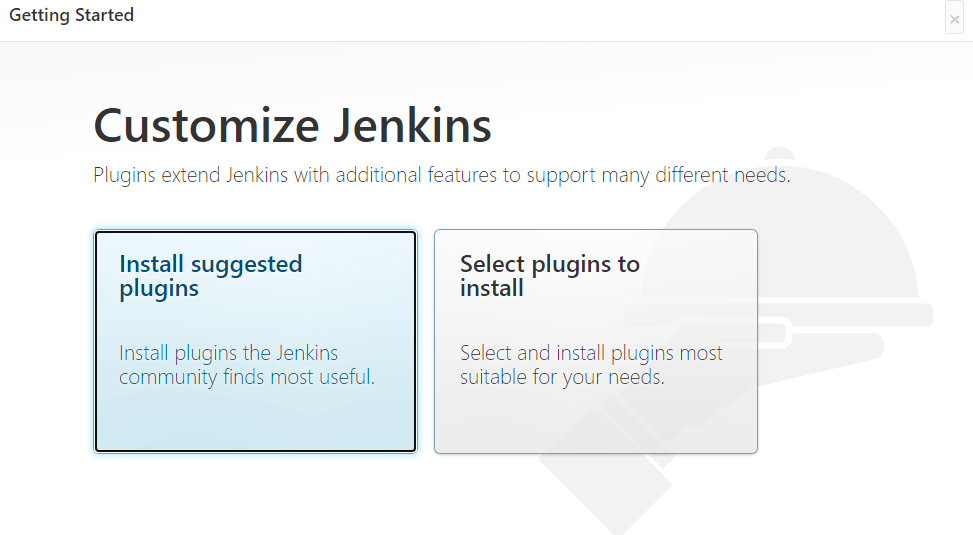
\includegraphics[width=15cm]{images-aws/24-jenkins-select-plugin.png}
        \caption{Customize Jenkins}
\end{figure}


4. We search for the \textbf{GitHub} plugin, select it and install.

\begin{figure}[h!]
    \centering
        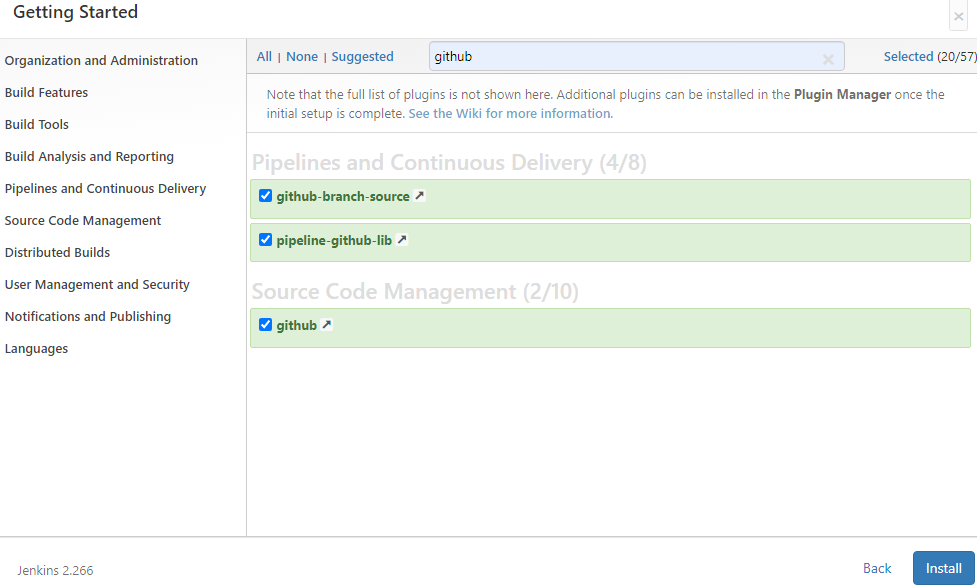
\includegraphics[width=15cm]{images-aws/25-jenkins-select-github-plugin.png}
        \caption{Select GitHub Plugin to be Installed}
\end{figure}




5. Once the installations is completed, we enter Administrator Credentials and click \textbf{Save and Continue}.

\begin{figure}[h!]
    \centering
        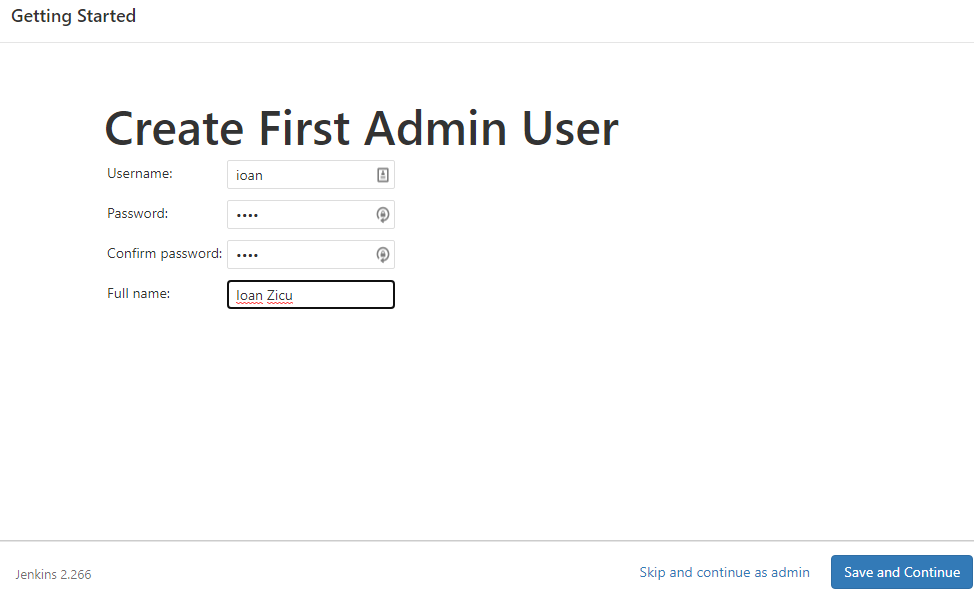
\includegraphics[width=15cm]{images-aws/26-jenkins-admin-user.png}
        \caption{Create First Admin User}
\end{figure}





6. Next window is \textbf{Instance Configuration} where we can see the Jenkins URL. We click \textbf{Save and Finish}.

\begin{figure}[h!]
    \centering
        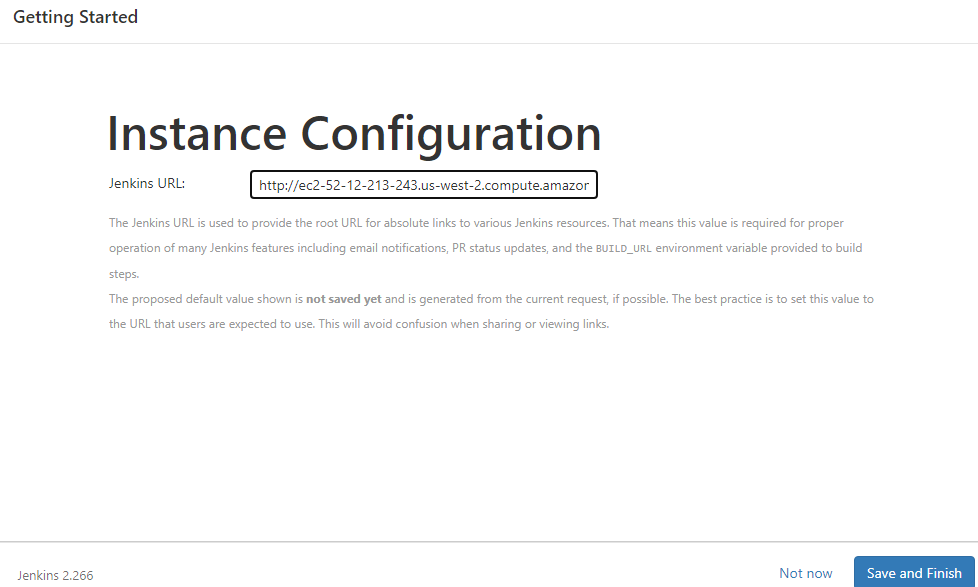
\includegraphics[width=15cm]{images-aws/27-jenkins-conf.png}
        \caption{Instance Configuration}
\end{figure}


At this moment we have completed the Jenkins setup.

\begin{figure}[h!]
    \centering
        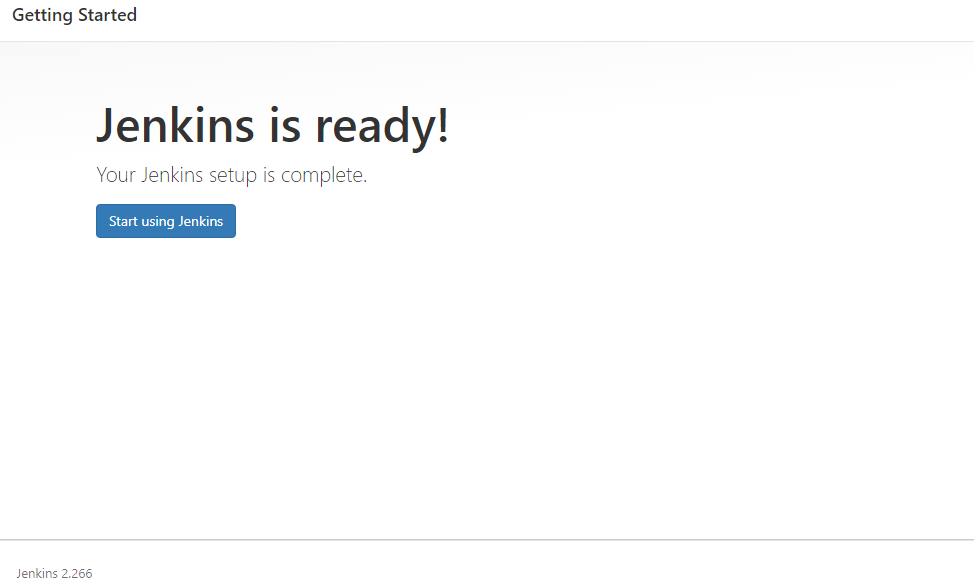
\includegraphics[width=15cm]{images-aws/28-jenkins-ready.png}
        \caption{Jenkins is Ready}
\end{figure}



\begin{figure}[h!]
    \centering
        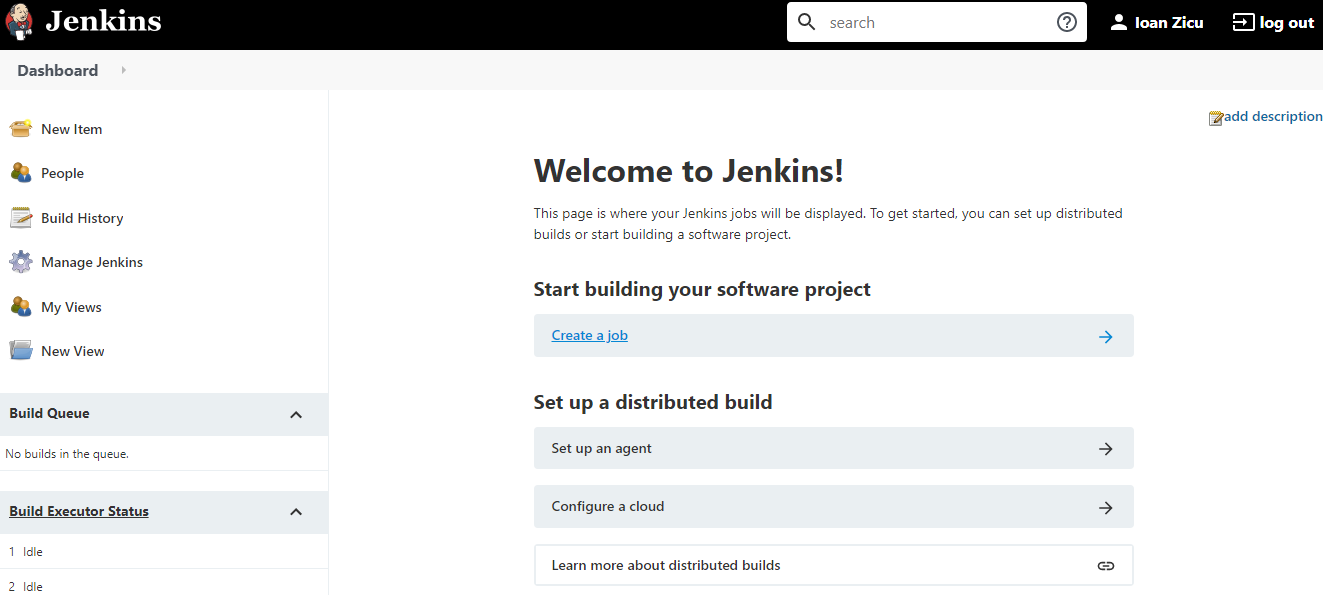
\includegraphics[width=15cm]{images-aws/30-jenkins-create-job.png}
        \caption{Welcome to Jenkins}
\end{figure}


\begin{figure}[h!]
    \centering
        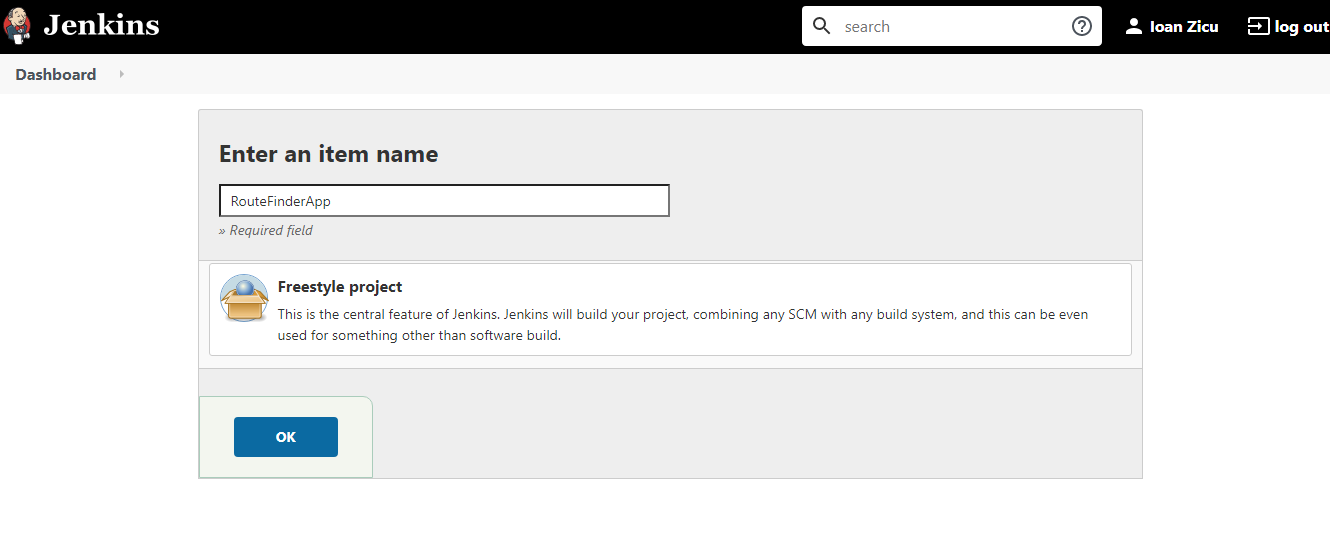
\includegraphics[width=15cm]{images-aws/31-jenkins-set-project-name.png}
        \caption{Create Jenkins Job}
\end{figure}


\begin{figure}[h!]
    \centering
        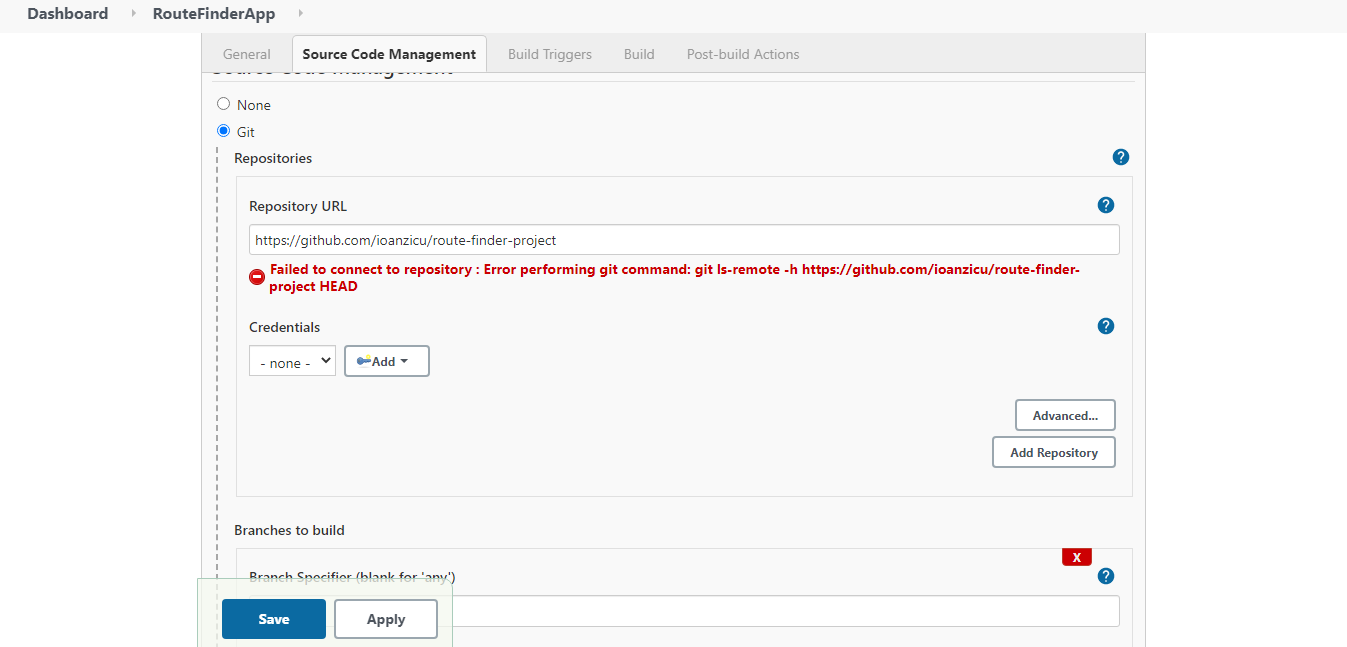
\includegraphics[width=15cm]{images-aws/32-jenkins-setup-repo.png}
        \caption{Setup GitHub Repository - Error}
\end{figure}


\begin{figure}[h!]
    \centering
        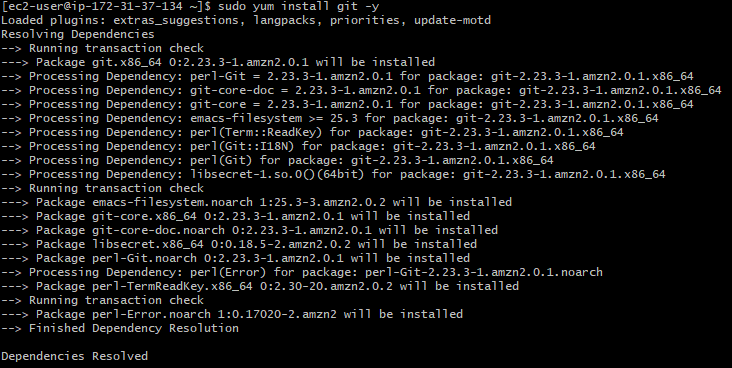
\includegraphics[width=15cm]{images-aws/33-jenkins-install-git.png}
        \caption{Install Git}
\end{figure}


\begin{figure}[h!]
    \centering
        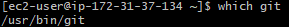
\includegraphics[width=6cm]{images-aws/34-jenkins-git-on-local.png}
        \caption{Get Jenkins location}
\end{figure}


\begin{figure}[h!]
    \centering
        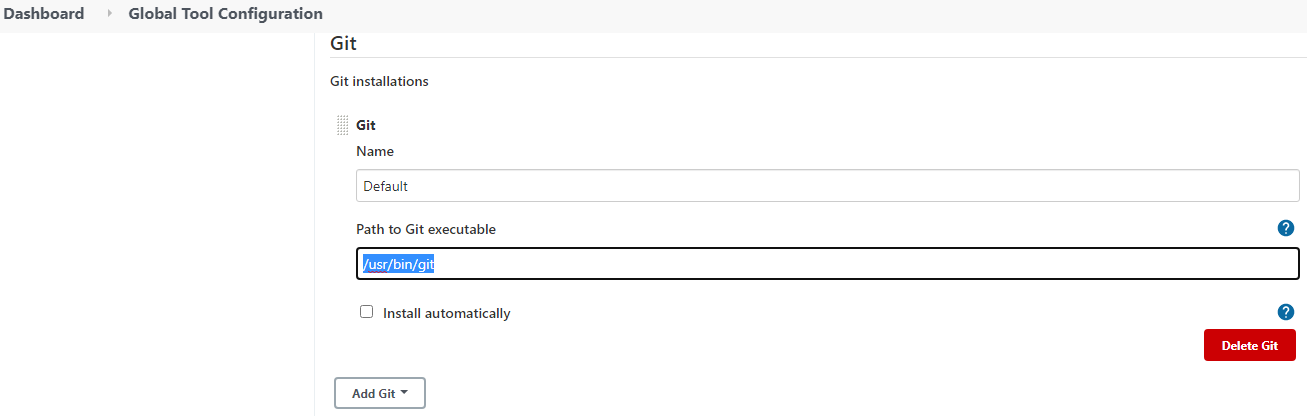
\includegraphics[width=15cm]{images-aws/36-jenkins-git-set-path.png}
        \caption{Setup the Git path to executable}
\end{figure}


\begin{figure}[h!]
    \centering
        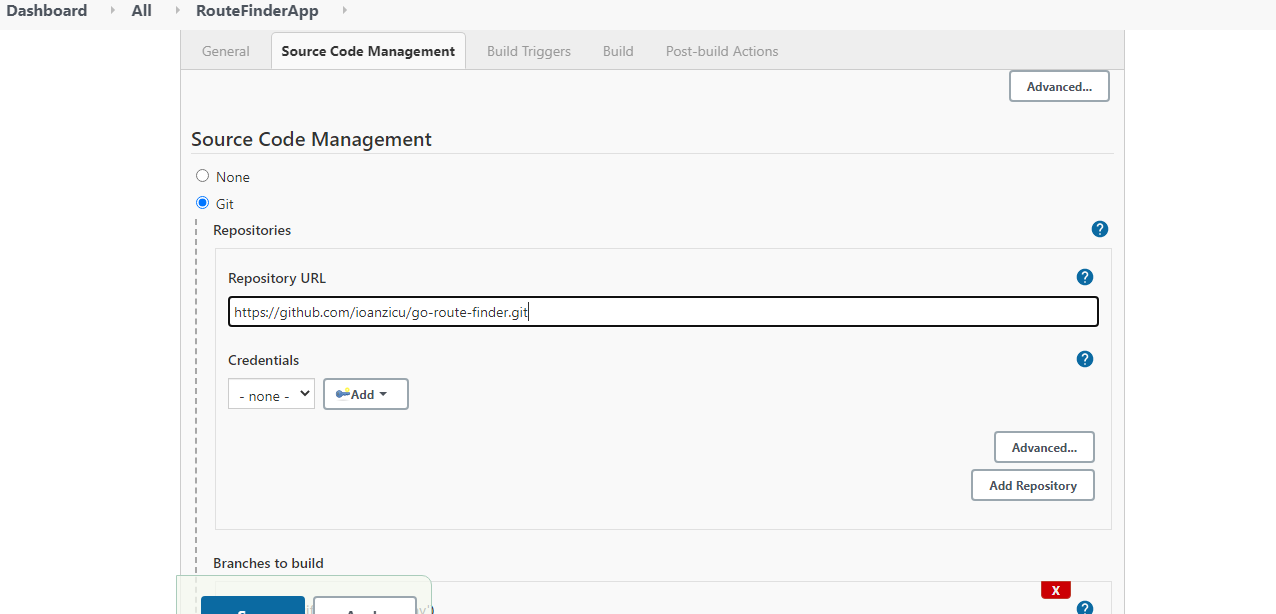
\includegraphics[width=15cm]{images-aws/37-jenkins-setup-repo-no-error.png}
        \caption{Setup GitHub Repository - No Error}
\end{figure}


\begin{figure}[h!]
    \centering
        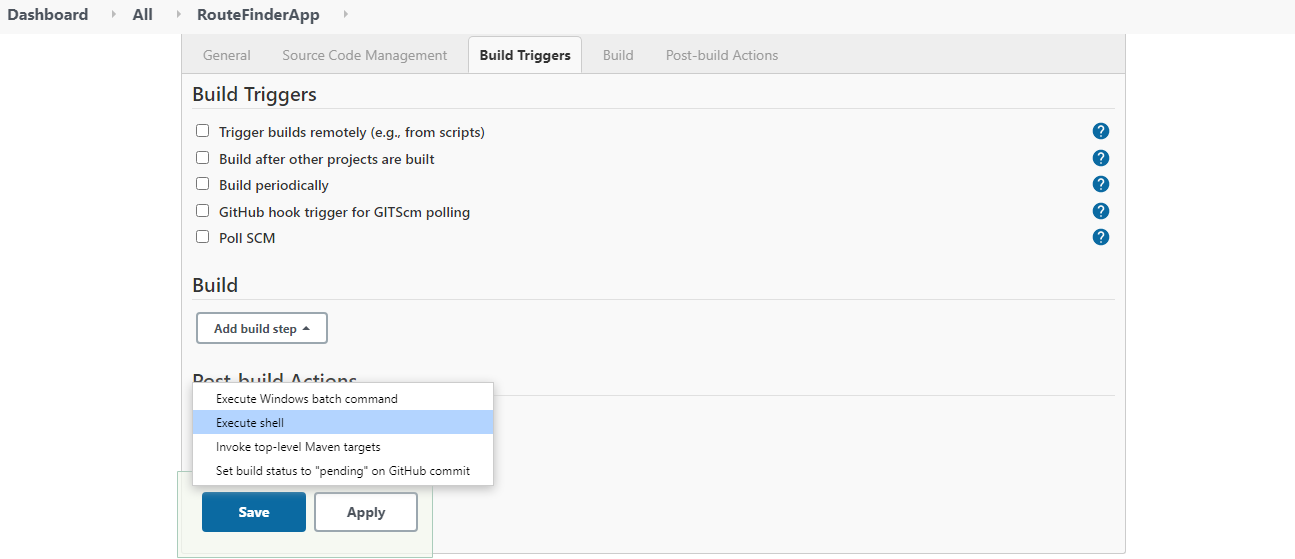
\includegraphics[width=15cm]{images-aws/38-jenkins-build-setup.png}
        \caption{Setup Build Triggers}
\end{figure}


\begin{figure}[h!]
    \centering
        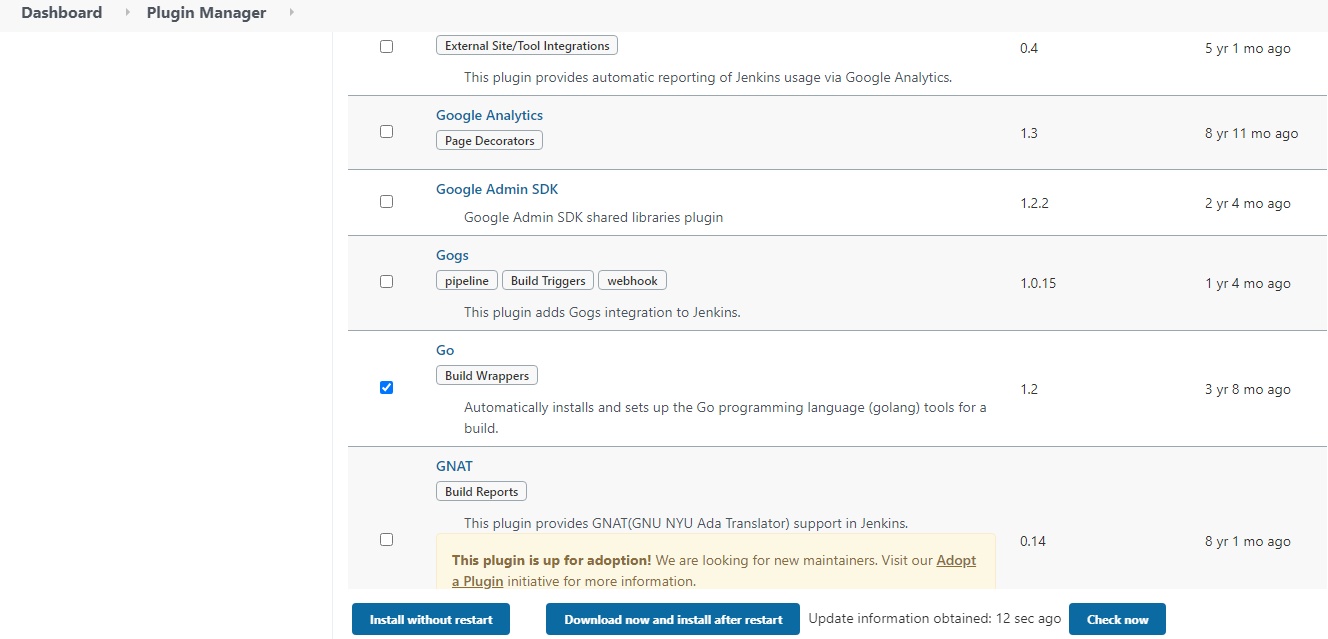
\includegraphics[width=15cm]{images-aws/39-go-plugin.png}
        \caption{Setup Plugin for the Golang Programming Language}
\end{figure}


\begin{figure}[h!]
    \centering
        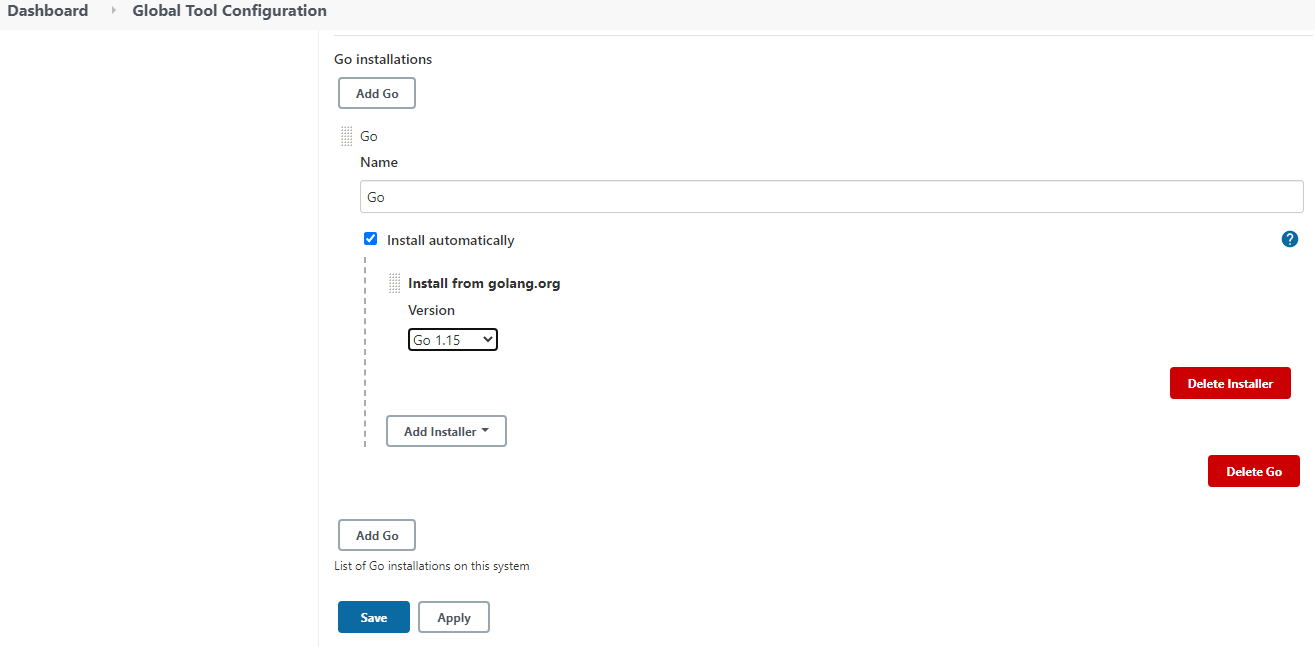
\includegraphics[width=15cm]{images-aws/41-go-global-tool.png}
        \caption{Configure Golang Version}
\end{figure}


\begin{figure}[h!]
    \centering
        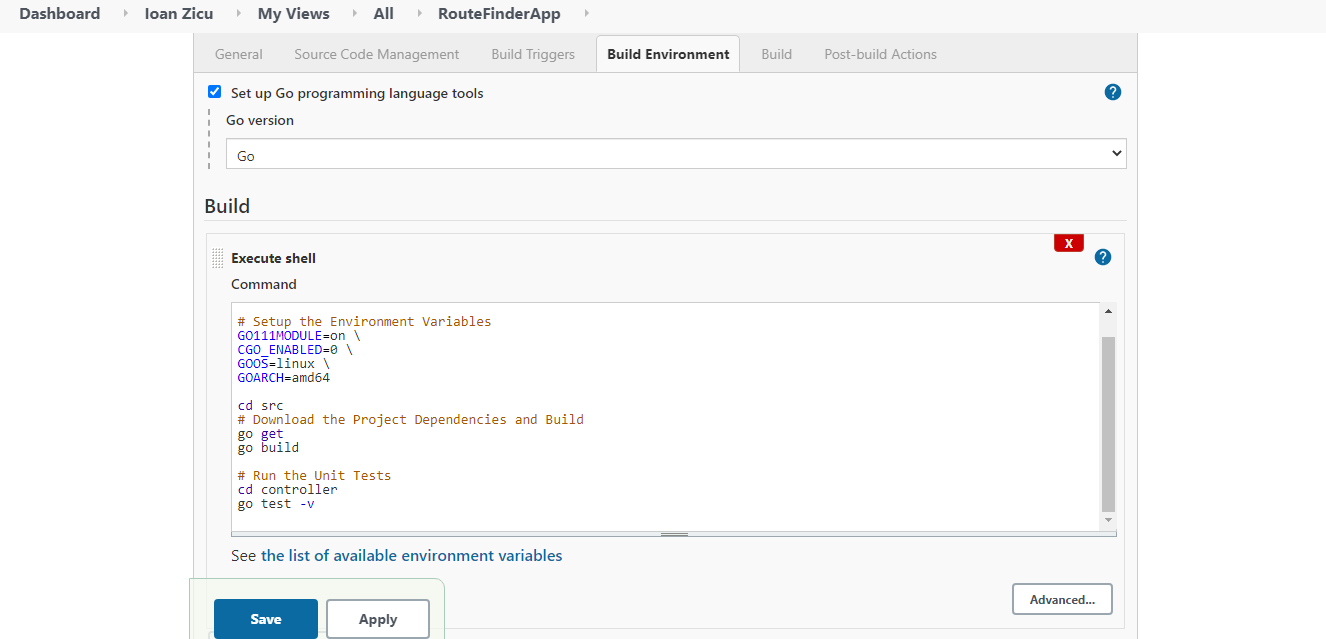
\includegraphics[width=15cm]{images-aws/42-project-build-env-golang-.png}
        \caption{Setup the Script for Build Environment}
\end{figure}

\begin{figure}[h!]
    \centering
        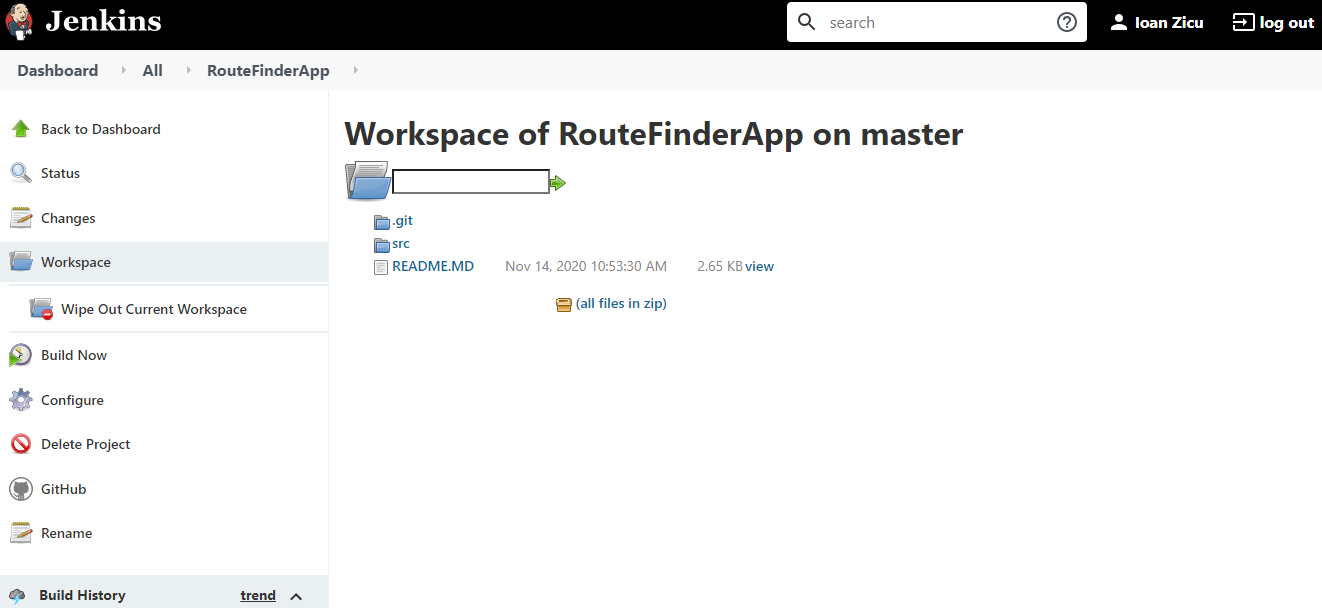
\includegraphics[width=15cm]{images-aws/44-project-workspace-git.png}
        \caption{Project Work Space}
\end{figure}


\begin{figure}[h!]
    \centering
        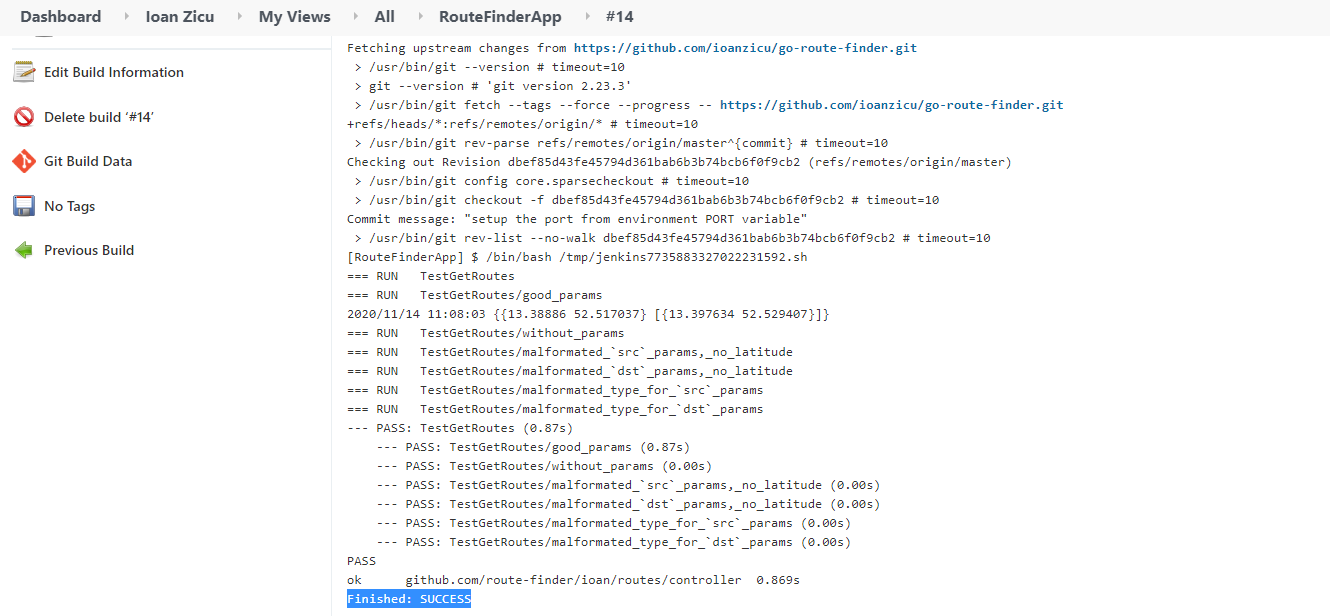
\includegraphics[width=15cm]{images-aws/45-test-build-.png}
        \caption{Run the Project Build}
\end{figure}


\begin{figure}[h!]
    \centering
        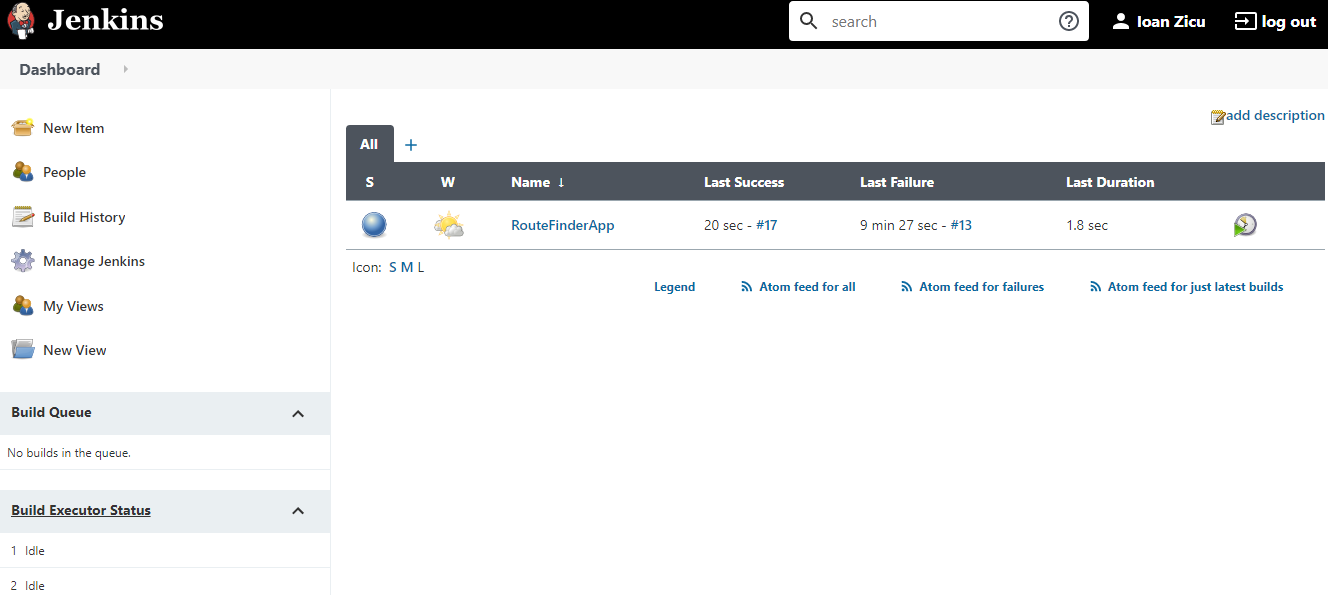
\includegraphics[width=15cm]{images-aws/46-test-build-success-.png}
        \caption{Project Status}
\end{figure}


\begin{figure}[h!]
    \centering
        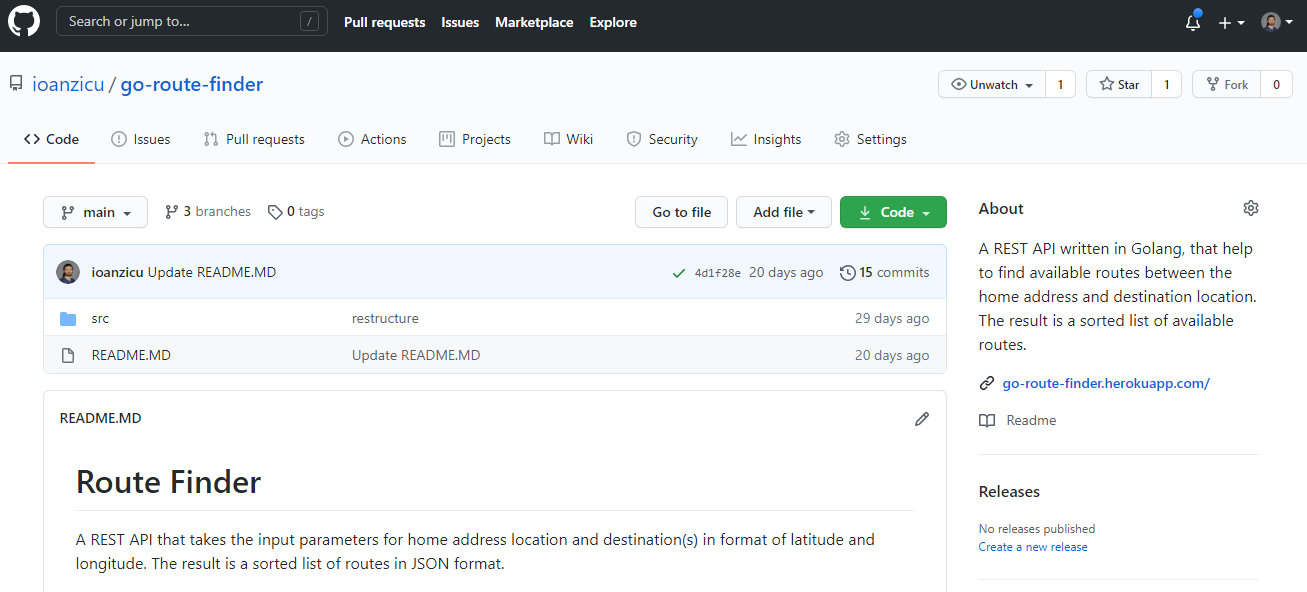
\includegraphics[width=15cm]{images-aws/47---github-project.png}
        \caption{RouteFinder Application GitHub Repository}
\end{figure}


\begin{figure}[h!]
    \centering
        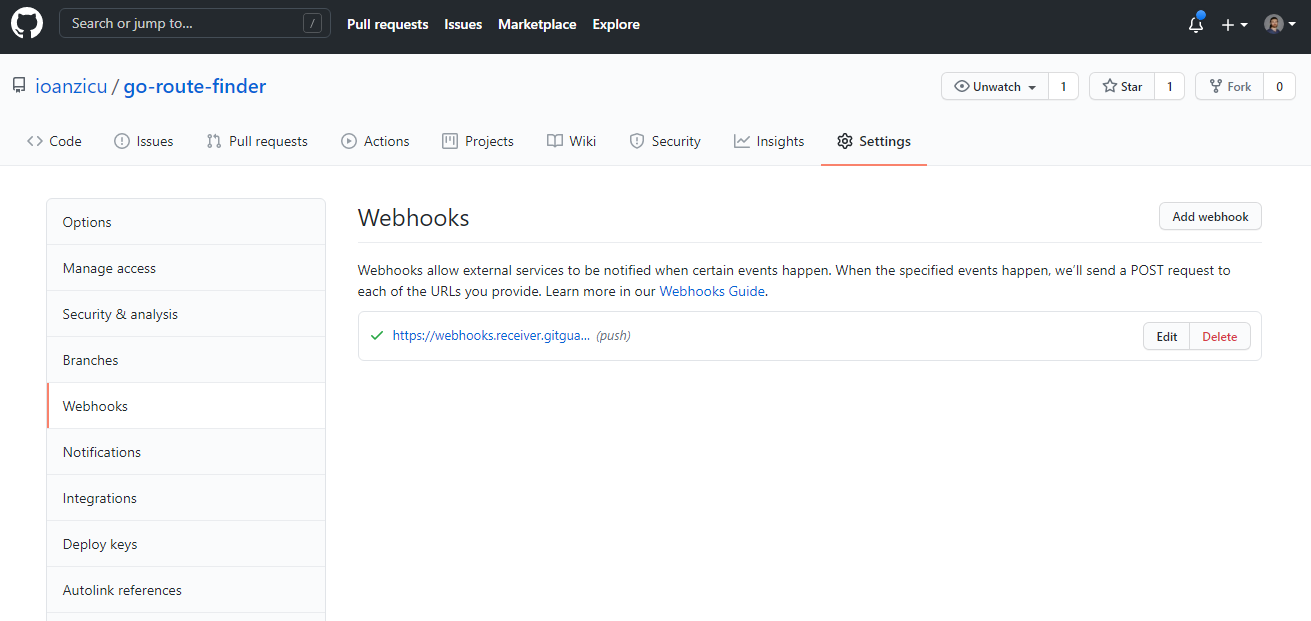
\includegraphics[width=15cm]{images-aws/48---web-hook.png}
        \caption{Check the Webhooks}
\end{figure}


\begin{figure}[h!]
    \centering
        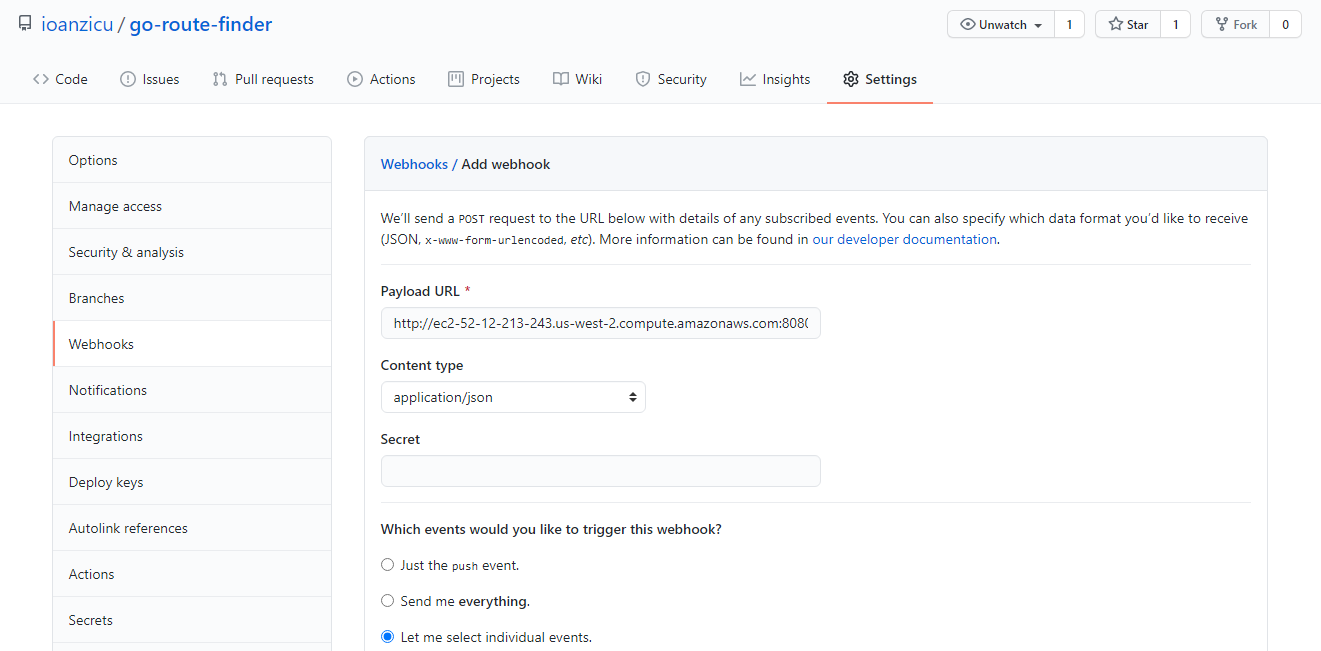
\includegraphics[width=15cm]{images-aws/49---web-hook-setup.png}
        \caption{Add new Webhook to trigger the Jenkins Build}
\end{figure}


\begin{figure}[h!]
    \centering
        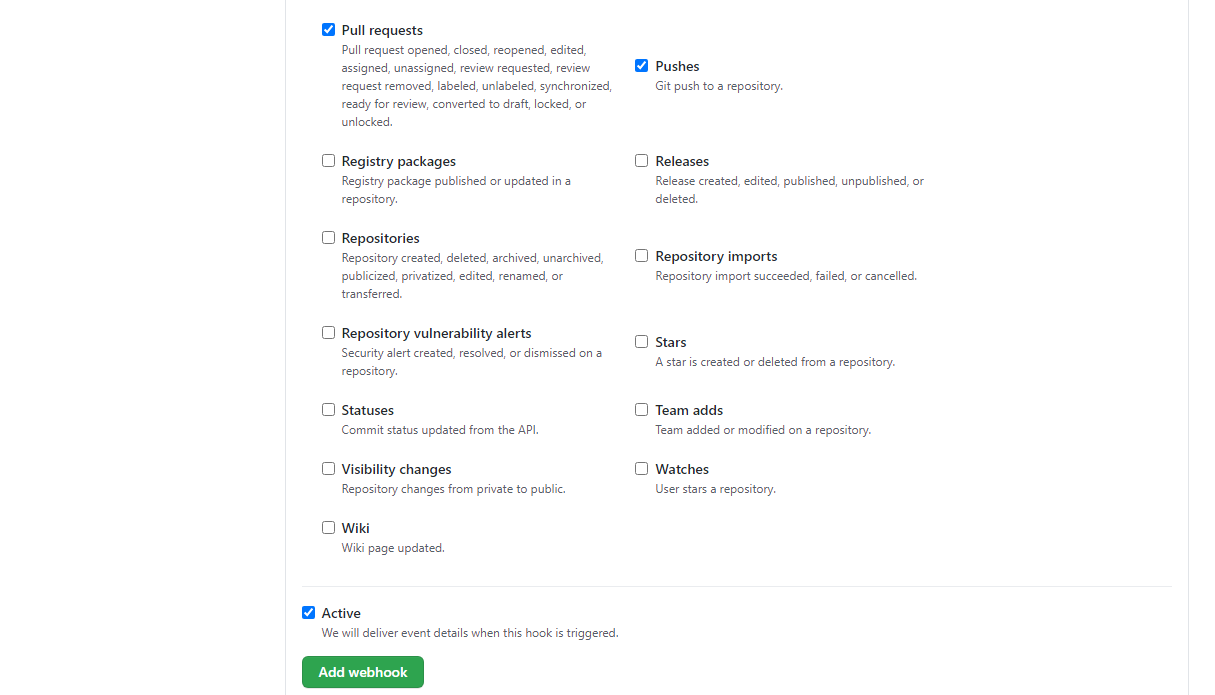
\includegraphics[width=15cm]{images-aws/50---web-hook-setup-pull.png}
        \caption{Trigger the Jenkins Build on Push and Pull Request}
\end{figure}


\begin{figure}[h!]
    \centering
        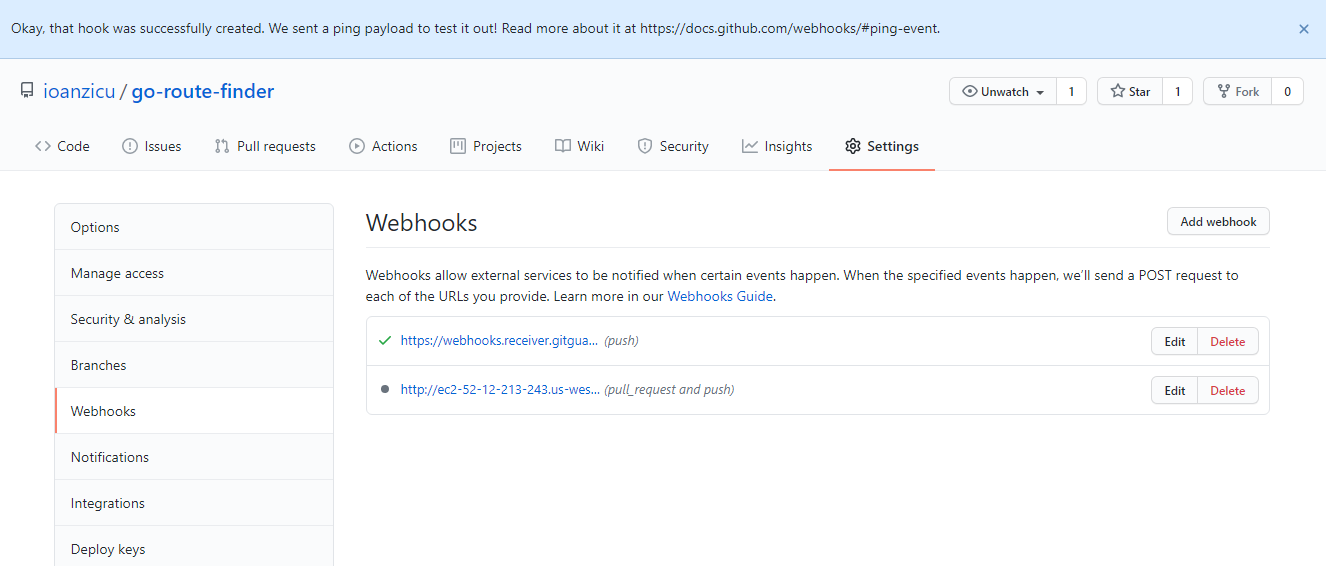
\includegraphics[width=15cm]{images-aws/51---web-hook-created.png}
        \caption{Webhook successfully created}
\end{figure}



\begin{figure}[h!]
    \centering
        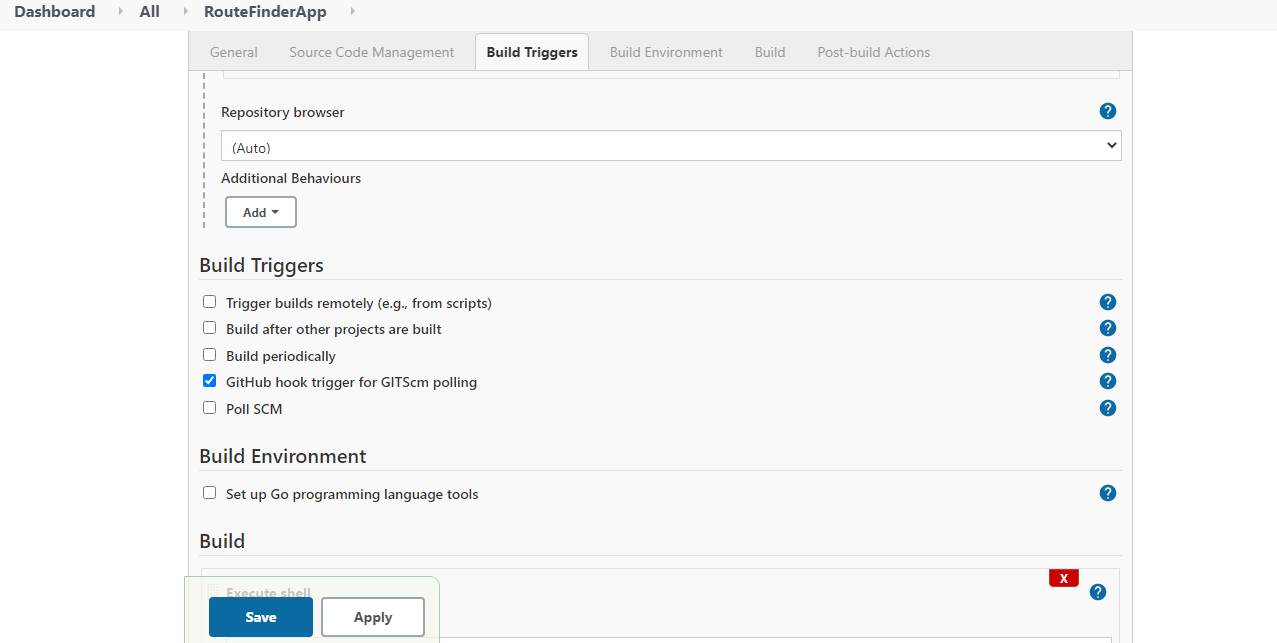
\includegraphics[width=15cm]{images-aws/52---trigger-jenkins.png}
        \caption{Setup the Github hook trigger for GITScm polling}
\end{figure}




\begin{figure}[h!]
    \centering
        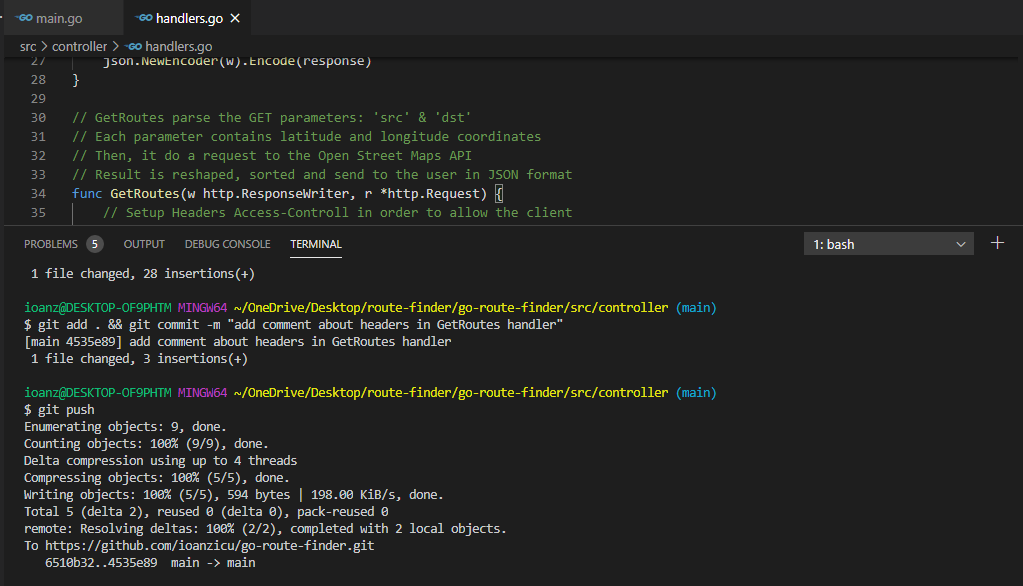
\includegraphics[width=15cm]{images-aws/53--small-commit-after-fixed-branches.png}
        \caption{Commit and Push a new Commit}
\end{figure}



\begin{figure}[h!]
    \centering
        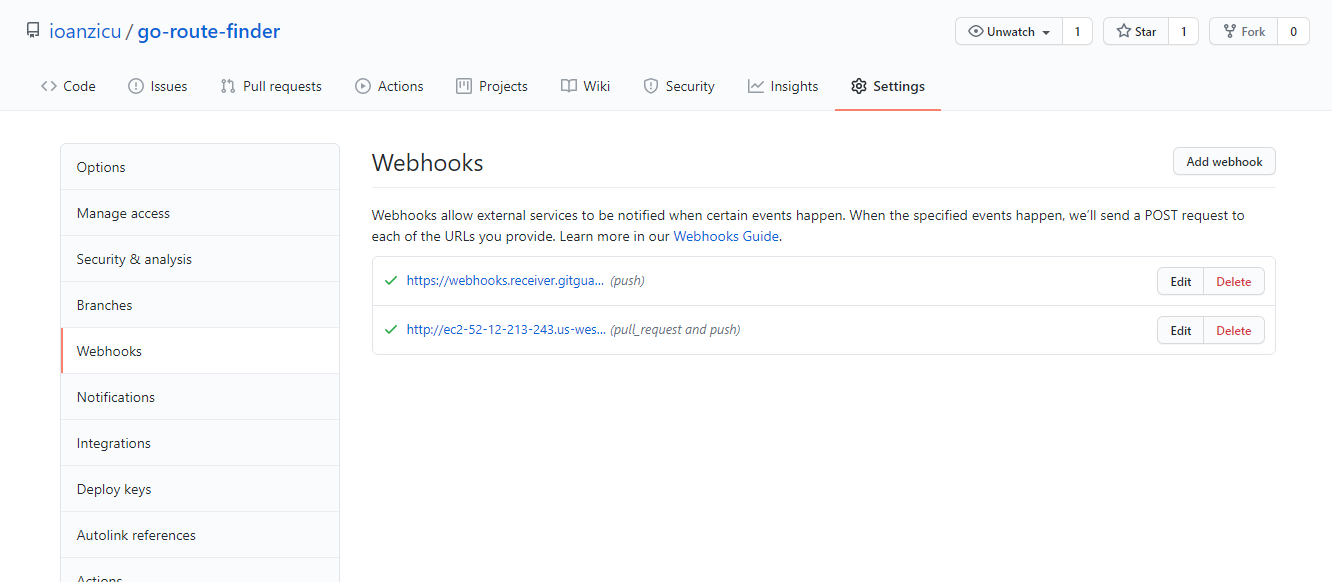
\includegraphics[width=15cm]{images-aws/54---successfull-push-webhook.png}
        \caption{Github hook is activated}
\end{figure}


\begin{figure}[h!]
    \centering
        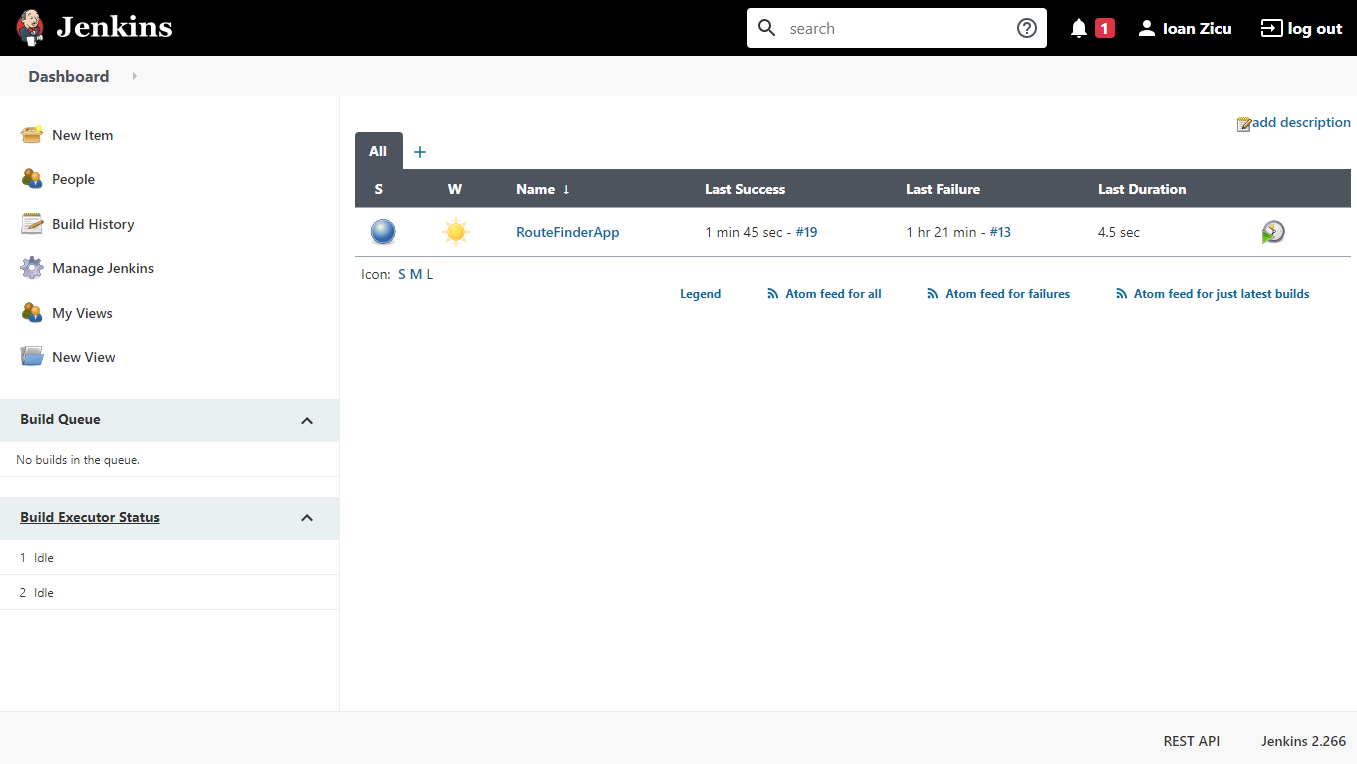
\includegraphics[width=15cm]{images-aws/55--triggered-push-3.png}
        \caption{Project status build - Last Success 1 minute 45 seconds ago}
\end{figure}


\begin{figure}[h!]
    \centering
        \includegraphics[width=10cm]{images-aws/56--triggered-push-4.png}
        \caption{Build Logs from the Console Output}
\end{figure}



















\newpage

\begin{thebibliography}{100}



% Setup azure Ubuntu VM
	\bibitem{} \url{https://docs.microsoft.com/en-us/azure/developer/jenkins/configure-on-linux-vm}

% Install Docker on Ubuntu VM
	\bibitem{} \url{https://docs.docker.com/engine/install/ubuntu/}

% Install Jenkins using Docker
	\bibitem{} \url{https://www.jenkins.io/doc/book/installing/docker/}

% Enable the port on Firewall
	\bibitem{} \url{https://www.digitalocean.com/community/tutorials/how-to-install-jenkins-on-ubuntu-18-04}

% New image
	\bibitem{} \url{https://hub.docker.com/r/jenkins/jenkins/}

% Github source
	\bibitem{} \url{https://github.com/jenkinsci/docker}


% Go Jenkins
	\bibitem{} \url{https://bmuschko.com/blog/go-on-jenkins/#:~:text=Jenkins}

% Pull Request
	\bibitem{} \url{https://devopscube.com/jenkins-build-trigger-github-pull-request/}


	\bibitem{} \url{https://www.blazemeter.com/blog/how-to-integrate-your-github-repository-to-your-jenkins-project}



\end{thebibliography}



\end{document}